\section{复变函数的积分}

其实就是关于某个参数 $\gamma:[0,1]\to C$ 进行积分
\[
\int_{\gamma}^{} f(z) \, dz =\int_{0}^{1} f(\gamma(t))\cdot\gamma'(t)  \, dt 
\]
柯西积分公式:若 $f$ 在一个包含圆周 $C$ 的区域内全纯,那么对于任意 $C$ 内的 $z$ 点,有
\begin{equation}
f(z)=\frac{1}{2\pi i}\int_{C}^{} \frac{f(\zeta)}{\zeta-z} \, d\zeta
\label{b51110}
\end{equation}

这个公式具有极其广泛的应用场景,比如计算导数,估计不等式....

\cref{b51110} 的证明思路就是类似于调和方程的平均值公式证明
\[
\int_{C}^{} \frac{f(\zeta)}{\zeta-z} \, d\zeta=\int_{C_{\epsilon}^{-}}^{} \frac{f(\zeta)}{\zeta-z} \, d\zeta \approx -f(z)\int_{0}^{2\pi} \frac{\epsilon ie^{ it }}{\epsilon e^{ it }} \, dt=-2\pi if(z)   
\]
对于 \cref{b51110} 两边同时求 $n$ 阶导数得到
\begin{equation}
f^{(n)}(z)=\frac{n!}{2\pi i}\int_{C}^{} \frac{f(\zeta)}{(\zeta-z)^{n+1}} \, d\zeta
\label{e4a292}
\end{equation}

这只需要根据导数的定义归纳验证导数的存在性即可.

柯西不等式 \cref{4ec030} 是 \cref{e4a292} 的直接推论
\begin{equation}
\lvert f^{(n)}(z_0) \rvert \leq \frac{n!\cdot \lVert f \rVert _{C}}{R^{n}}\qquad \text{where }\lVert f \rVert _{C}\coloneqq \sup_{z\in C}\lvert f(z) \rvert
\label{4ec030}
\end{equation}

进一步我们有复变函数的幂级数表示
\begin{equation}
\begin{aligned}
f(z) & =\frac{1}{2\pi i}\int_{C}^{} \frac{f(\zeta)}{\zeta-z} \, d\zeta=\frac{1}{2\pi i} \int_{C}^{} \frac{f(\zeta)}{\zeta-z_0} \sum_{n=0}^{\infty} \left( \frac{z-z_0}{\zeta-z_0} \right)^{n} \, d\zeta    \\
 & =\sum_{n=0}^{\infty }\left( \frac{1}{2\pi i} \int_{C}^{} \frac{f(\zeta)}{(\zeta-z_0)^{n+1}} \, d\zeta  \right)\cdot(z-z_0)^{n}  
\end{aligned}
\label{945f8c}
\end{equation}

同时还有 Liouville 定理:若 $f$ 全纯且有界,那么 $f$ 是常值函数. (直接利用 \cref{e4a292} )
\[
\lvert f'(z) \rvert =\left\lvert  \frac{1}{2\pi i}\int_{C_{R}}^{} \frac{f(\zeta)}{(\zeta-z)^{2}} \, d\zeta   \right\rvert  \leq \frac{1}{2\pi}\int_{C_{R}}^{} \frac{M}{R^2} \, dz=\frac{M}{R}  \to0\qquad \text{as }R\to \infty
\]
然后可以证明代数基本定理.

根据幂级数表示 \cref{945f8c}  可以证明复变函数的零点集是离散的.

\subsection{积分估计}

参见《复变函数论 》(第五版) 学习指导书 (钟玉泉编).

已知 Jordan 不等式
\[
\frac{2\theta}{\pi}\leq \sin\theta\leq \theta \qquad \theta\in\left[ 0,\frac{\pi}{2} \right]
\]
证明:
\begin{equation}
\left\lvert  \int_{C}^{} e^{ iz }  \, \mathrm{d}z   \right\rvert <\pi
\label{3ab879}
\end{equation}

其中 $C$ 为圆周 $\lvert z \rvert=R$ 的上半圆周从 $R$ 到 $-R$.

选取参数化 $C:z=R e^{ i\theta },\theta\in[0,\pi]$. 于是
\[
\begin{aligned}
\left\lvert  \int_{C}^{} e^{ iz } \, \mathrm{d}z   \right\rvert  & \leq \int_{C}^{} \lvert e^{ iz } \rvert  \, \lvert \mathrm{d}z \rvert  =\int_{0}^{\pi} e^{ -R\sin\theta }R \, \mathrm{d}\theta\\
 & =2\int_{0}^{\pi/2 } e^{ -R\sin\theta }R \, \mathrm{d}\theta \leq 2\int_{0}^{\pi/2 } e^{ -2R\theta/\pi  }R \, \mathrm{d}\theta \\
 & =-\pi \left.e^{ -2R\theta/\pi }\right|^{\pi/2 }_{0}=\pi (1-e^{ -R })<\pi 
\end{aligned}
\]
\begin{remark}
不等式 \cref{3ab879}  是一个重要不等式. 可以用来放缩很多围道积分(用来证明 Jordan 引理 )
\end{remark}
\begin{exercise}
若 $I_{r}=\int_{C_{r}}^{} \frac{e^{ iz }}{z} \, \mathrm{d}z$,其中 $C_{r}$ 是从 $r$ 到 $-r$ 沿 $\lvert z \rvert=r$ 的上半圆周,证明:
\[
\lim_{ r \to +\infty } I_{r}=0\qquad \lim_{ r \to 0 } I_{r}=\pi i
\]
\end{exercise}
\begin{proof}
$r\to +\infty$ 时,直接利用 \cref{3ab879} 放缩
\[
\lvert I_{r} \rvert \leq \frac{\pi }{r}\to0
\]
$r\to0$ 时,利用留数定理显然,或者直接放缩估计 $\lvert I_{r}-\pi i \rvert\to0$.

\end{proof}

\subsection{柯西积分定理}
\[
f(z)=\frac{1}{2\pi i}\oint_{C} \frac{f(\zeta)}{\zeta-z} \, \mathrm{d}\zeta \qquad z\text{在}C\text{内部}  
\]
柯西积分定理对于解析函数 $f(z)$ 的实部和虚部都不成立.

对于一般的题目,正常计算即可. 注意先将分母有理化,再判断奇点是否在积分曲线内部.

下面介绍一种思想:
\begin{figure}[H]
\centering
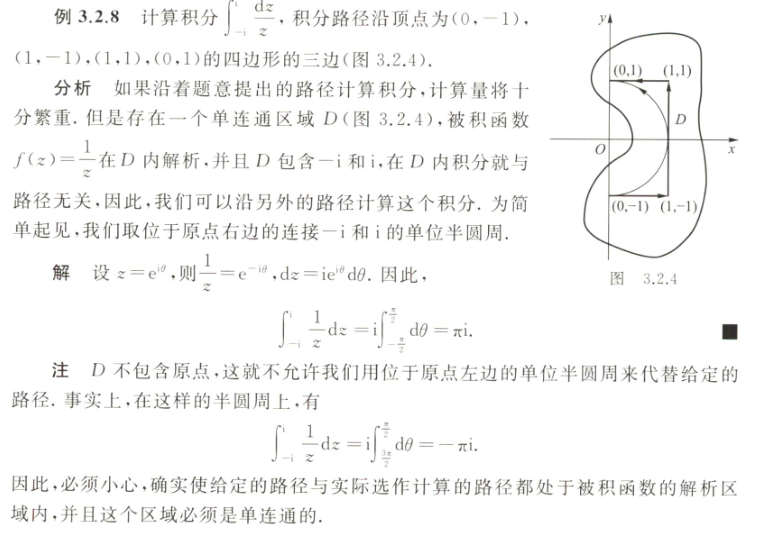
\includegraphics[width=\textwidth]{复变函数的积分-2025040601.png}
% \caption{}
\label{}
\end{figure}
